\documentclass[a4paper,11pt]{article}
\usepackage[a4paper, margin=8em]{geometry}

% usa i pacchetti per la scrittura in italiano
\usepackage[french,italian]{babel}
\usepackage[T1]{fontenc}
\usepackage[utf8]{inputenc}
\frenchspacing 

% usa i pacchetti per la formattazione matematica
\usepackage{amsmath, amssymb, amsthm, amsfonts}

% usa altri pacchetti
\usepackage{gensymb}
\usepackage{hyperref}
\usepackage{standalone}

\usepackage{colortbl}

\usepackage{xstring}
\usepackage{karnaugh-map}

% imposta il titolo
\title{Appunti Ingegneria del Software}
\author{Luca Seggiani}
\date{2025}

% imposta lo stile
% usa helvetica
\usepackage[scaled]{helvet}
% usa palatino
\usepackage{palatino}
% usa un font monospazio guardabile
\usepackage{lmodern}

\renewcommand{\rmdefault}{ppl}
\renewcommand{\sfdefault}{phv}
\renewcommand{\ttdefault}{lmtt}

% circuiti
\usepackage{circuitikz}
\usetikzlibrary{babel}

% testo cerchiato
\newcommand*\circled[1]{\tikz[baseline=(char.base)]{
            \node[shape=circle,draw,inner sep=2pt] (char) {#1};}}

% disponi il titolo
\makeatletter
\renewcommand{\maketitle} {
	\begin{center} 
		\begin{minipage}[t]{.8\textwidth}
			\textsf{\huge\bfseries \@title} 
		\end{minipage}%
		\begin{minipage}[t]{.2\textwidth}
			\raggedleft \vspace{-1.65em}
			\textsf{\small \@author} \vfill
			\textsf{\small \@date}
		\end{minipage}
		\par
	\end{center}

	\thispagestyle{empty}
	\pagestyle{fancy}
}
\makeatother

% disponi teoremi
\usepackage{tcolorbox}
\newtcolorbox[auto counter, number within=section]{theorem}[2][]{%
	colback=blue!10, 
	colframe=blue!40!black, 
	sharp corners=northwest,
	fonttitle=\sffamily\bfseries, 
	title=Teorema~\thetcbcounter: #2, 
	#1
}

% disponi definizioni
\newtcolorbox[auto counter, number within=section]{definition}[2][]{%
	colback=red!10,
	colframe=red!40!black,
	sharp corners=northwest,
	fonttitle=\sffamily\bfseries,
	title=Definizione~\thetcbcounter: #2,
	#1
}

% disponi codice
\usepackage{listings}
\usepackage[table]{xcolor}

\definecolor{codegreen}{rgb}{0,0.6,0}
\definecolor{codegray}{rgb}{0.5,0.5,0.5}
\definecolor{codepurple}{rgb}{0.58,0,0.82}
\definecolor{backcolour}{rgb}{0.95,0.95,0.92}

\lstdefinestyle{codestyle}{
		backgroundcolor=\color{black!5}, 
		commentstyle=\color{codegreen},
		keywordstyle=\bfseries\color{magenta},
		numberstyle=\sffamily\tiny\color{black!60},
		stringstyle=\color{green!50!black},
		basicstyle=\ttfamily\footnotesize,
		breakatwhitespace=false,         
		breaklines=true,                 
		captionpos=b,                    
		keepspaces=true,                 
		numbers=left,                    
		numbersep=5pt,                  
		showspaces=false,                
		showstringspaces=false,
		showtabs=false,                  
		tabsize=2
}

\lstdefinestyle{shellstyle}{
		backgroundcolor=\color{black!5}, 
		basicstyle=\ttfamily\footnotesize\color{black}, 
		commentstyle=\color{black}, 
		keywordstyle=\color{black},
		numberstyle=\color{black!5},
		stringstyle=\color{black}, 
		showspaces=false,
		showstringspaces=false, 
		showtabs=false, 
		tabsize=2, 
		numbers=none, 
		breaklines=true
}


\lstdefinelanguage{assembler}{ 
  keywords={AAA, AAD, AAM, AAS, ADC, ADCB, ADCW, ADCL, ADD, ADDB, ADDW, ADDL, AND, ANDB, ANDW, ANDL,
        ARPL, BOUND, BSF, BSFL, BSFW, BSR, BSRL, BSRW, BSWAP, BT, BTC, BTCB, BTCW, BTCL, BTR, 
        BTRB, BTRW, BTRL, BTS, BTSB, BTSW, BTSL, CALL, CBW, CDQ, CLC, CLD, CLI, CLTS, CMC, CMP,
        CMPB, CMPW, CMPL, CMPS, CMPSB, CMPSD, CMPSW, CMPXCHG, CMPXCHGB, CMPXCHGW, CMPXCHGL,
        CMPXCHG8B, CPUID, CWDE, DAA, DAS, DEC, DECB, DECW, DECL, DIV, DIVB, DIVW, DIVL, ENTER,
        HLT, IDIV, IDIVB, IDIVW, IDIVL, IMUL, IMULB, IMULW, IMULL, IN, INB, INW, INL, INC, INCB,
        INCW, INCL, INS, INSB, INSD, INSW, INT, INT3, INTO, INVD, INVLPG, IRET, IRETD, JA, JAE,
        JB, JBE, JC, JCXZ, JE, JECXZ, JG, JGE, JL, JLE, JMP, JNA, JNAE, JNB, JNBE, JNC, JNE, JNG,
        JNGE, JNL, JNLE, JNO, JNP, JNS, JNZ, JO, JP, JPE, JPO, JS, JZ, LAHF, LAR, LCALL, LDS,
        LEA, LEAVE, LES, LFS, LGDT, LGS, LIDT, LMSW, LOCK, LODSB, LODSD, LODSW, LOOP, LOOPE,
        LOOPNE, LSL, LSS, LTR, MOV, MOVB, MOVW, MOVL, MOVSB, MOVSD, MOVSW, MOVSX, MOVSXB,
        MOVSXW, MOVSXL, MOVZX, MOVZXB, MOVZXW, MOVZXL, MUL, MULB, MULW, MULL, NEG, NEGB, NEGW,
        NEGL, NOP, NOT, NOTB, NOTW, NOTL, OR, ORB, ORW, ORL, OUT, OUTB, OUTW, OUTL, OUTSB, OUTSD,
        OUTSW, POP, POPL, POPW, POPB, POPA, POPAD, POPF, POPFD, PUSH, PUSHL, PUSHW, PUSHB, PUSHA, 
				PUSHAD, PUSHF, PUSHFD, RCL, RCLB, RCLW, MOVSL, MOVSB, MOVSW, STOSL, STOSB, STOSW, LODSB, LODSW,
				LODSL, INSB, INSW, INSL, OUTSB, OUTSL, OUTSW
        RCLL, RCR, RCRB, RCRW, RCRL, RDMSR, RDPMC, RDTSC, REP, REPE, REPNE, RET, ROL, ROLB, ROLW,
        ROLL, ROR, RORB, RORW, RORL, SAHF, SAL, SALB, SALW, SALL, SAR, SARB, SARW, SARL, SBB,
        SBBB, SBBW, SBBL, SCASB, SCASD, SCASW, SETA, SETAE, SETB, SETBE, SETC, SETE, SETG, SETGE,
        SETL, SETLE, SETNA, SETNAE, SETNB, SETNBE, SETNC, SETNE, SETNG, SETNGE, SETNL, SETNLE,
        SETNO, SETNP, SETNS, SETNZ, SETO, SETP, SETPE, SETPO, SETS, SETZ, SGDT, SHL, SHLB, SHLW,
        SHLL, SHLD, SHR, SHRB, SHRW, SHRL, SHRD, SIDT, SLDT, SMSW, STC, STD, STI, STOSB, STOSD,
        STOSW, STR, SUB, SUBB, SUBW, SUBL, TEST, TESTB, TESTW, TESTL, VERR, VERW, WAIT, WBINVD,
        XADD, XADDB, XADDW, XADDL, XCHG, XCHGB, XCHGW, XCHGL, XLAT, XLATB, XOR, XORB, XORW, XORL},
  keywordstyle=\color{blue}\bfseries,
  ndkeywordstyle=\color{darkgray}\bfseries,
  identifierstyle=\color{black},
  sensitive=false,
  comment=[l]{\#},
  morecomment=[s]{/*}{*/},
  commentstyle=\color{purple}\ttfamily,
  stringstyle=\color{red}\ttfamily,
  morestring=[b]',
  morestring=[b]"
}

\lstset{language=assembler, style=codestyle}

% disponi sezioni
\usepackage{titlesec}

\titleformat{\section}
	{\sffamily\Large\bfseries} 
	{\thesection}{1em}{} 
\titleformat{\subsection}
	{\sffamily\large\bfseries}   
	{\thesubsection}{1em}{} 
\titleformat{\subsubsection}
	{\sffamily\normalsize\bfseries} 
	{\thesubsubsection}{1em}{}

% tikz
\usepackage{tikz}

% float
\usepackage{float}

% grafici
\usepackage{pgfplots}
\pgfplotsset{width=10cm,compat=1.9}

% disponi alberi
\usepackage{forest}

\forestset{
	rectstyle/.style={
		for tree={rectangle,draw,font=\large\sffamily}
	},
	roundstyle/.style={
		for tree={circle,draw,font=\large}
	}
}

% disponi algoritmi
\usepackage{algorithm}
\usepackage{algorithmic}
\makeatletter
\renewcommand{\ALG@name}{Algoritmo}
\makeatother

% disponi numeri di pagina
\usepackage{fancyhdr}
\fancyhf{} 
\fancyfoot[L]{\sffamily{\thepage}}

\makeatletter
\fancyhead[L]{\raisebox{1ex}[0pt][0pt]{\sffamily{\@title \ \@date}}} 
\fancyhead[R]{\raisebox{1ex}[0pt][0pt]{\sffamily{\@author}}}
\makeatother

\begin{document}
% sezione (data)
\section{Lezione del 10-10-25}

% stili pagina
\thispagestyle{empty}
\pagestyle{fancy}

% testo
\subsubsection{Ereditarietà multipla}
Torniamo al discorso dell'ereditarietà.
In UML è permessa l'\textbf{ereditarietà multipla}, in quanto questa esiste in linguaggi come il C++.
Spesso, però, questo rappresenta un pattern da evitare ed è considerato un errore di progetto.

In prospettiva che si verificheranno errori, infatti, è meglio mantenere lineari le catene di ereditarietà in modo da minimizzare problemi.

\subsection{Realizzazione casi d'uso}
Abbiamo discusso finora la \textit{modellazione delle classi di analisi}, che deve essere il primo artefatto generato dalla fase di analisi.
Veniamo adesso al secondo, cioè la \textbf{realizzazione dei casi d'uso}.

Se le classi rappresentavano l'aspetto \textbf{statico} del sistema, le realizzazioni dei casi d'uso ne rappresentano l'aspetto \textbf{dinamico}.

Gli obiettivi che ci prefissiamo sono:
\begin{itemize}
	\item Trovare quali classi interagiscono per realizzare il comportamento specificato da un caso d'uso;
	\item Trovare quali \textbf{messaggi} queste classi devono inviarsi per realizzare tale comportamento. In questo modo possiamo determinare quali \textit{operazioni}, \textit{attributi} e \textit{relazioni} le classi dovranno avere.
\end{itemize}

Per dettagliare questo comportamento sfruttiamo 4 diagrammi, che sono:
\begin{itemize}
	\item Diagrammi di \textbf{sequenza}: mostrano la sequenza di messaggi, dall'alto verso il basso, che due classi si scambiano per realizzare un comportamento;
	\item Diagrammi di \textbf{comunicazione}: mostrano le relazioni strutturali degli oggetti;
	\item Diagrammi di \textbf{visione generale dell'interazione}: mostrano come più comportamenti semplici implementano comportamenti complessi;
	\item Diagrammi di \textbf{temporizzazione}: mostrano gli aspetti in tempo reale di un'operazione.
\end{itemize}

\subsubsection{Linee di vita}
Una \textit{linea di vita} (\textbf{lifeline}) rappresenta un partecipante in un'interazione, e in particolare il \textit{ruolo} che tale partecipante intepreta in tale interazione.

Ogni linea di vita ha un nome (opzionale), un tipo e un selettore (opzionale). Il selettore è una condizione booleana che può essere usata per selezionare quali istanze partecipano all'interazione.

\subsubsection{Messaggi}
Un \textbf{messaggio} specifica una comunicazione fra due linee di vita in un'interazione.
La comunicazione può essere:
\begin{itemize}
	\item L'invocazione di un'operazione;
	\item La creazione o distruzione di un'istanza;
	\item L'invio di un segnale.
\end{itemize}

La freccia che rappresenta il messaggio può codificare diverse informazioni:
\begin{itemize}
	\item \textbf{Messaggi sincroni}, rappresentati da freccia piena, significano che il mittente si ferma ad aspettare che il ricevitore esegua il messaggio;
	\item \textbf{Messaggi asincroni}, rappresentati da freccia vuota, significano che il mittente non si ferma ad aspettare il ricevitore ma prosegue;
\end{itemize}

Esistono poi altri modelli che rappresentano informazioni come il \textit{messaggio di ritorno}, la \textit{creazione o distruzione di oggetti}, ecc...

Vediamo quindi un esempio di due linee vita associate a \textit{classi} che si scambiano messaggi in UML:
\begin{center}
	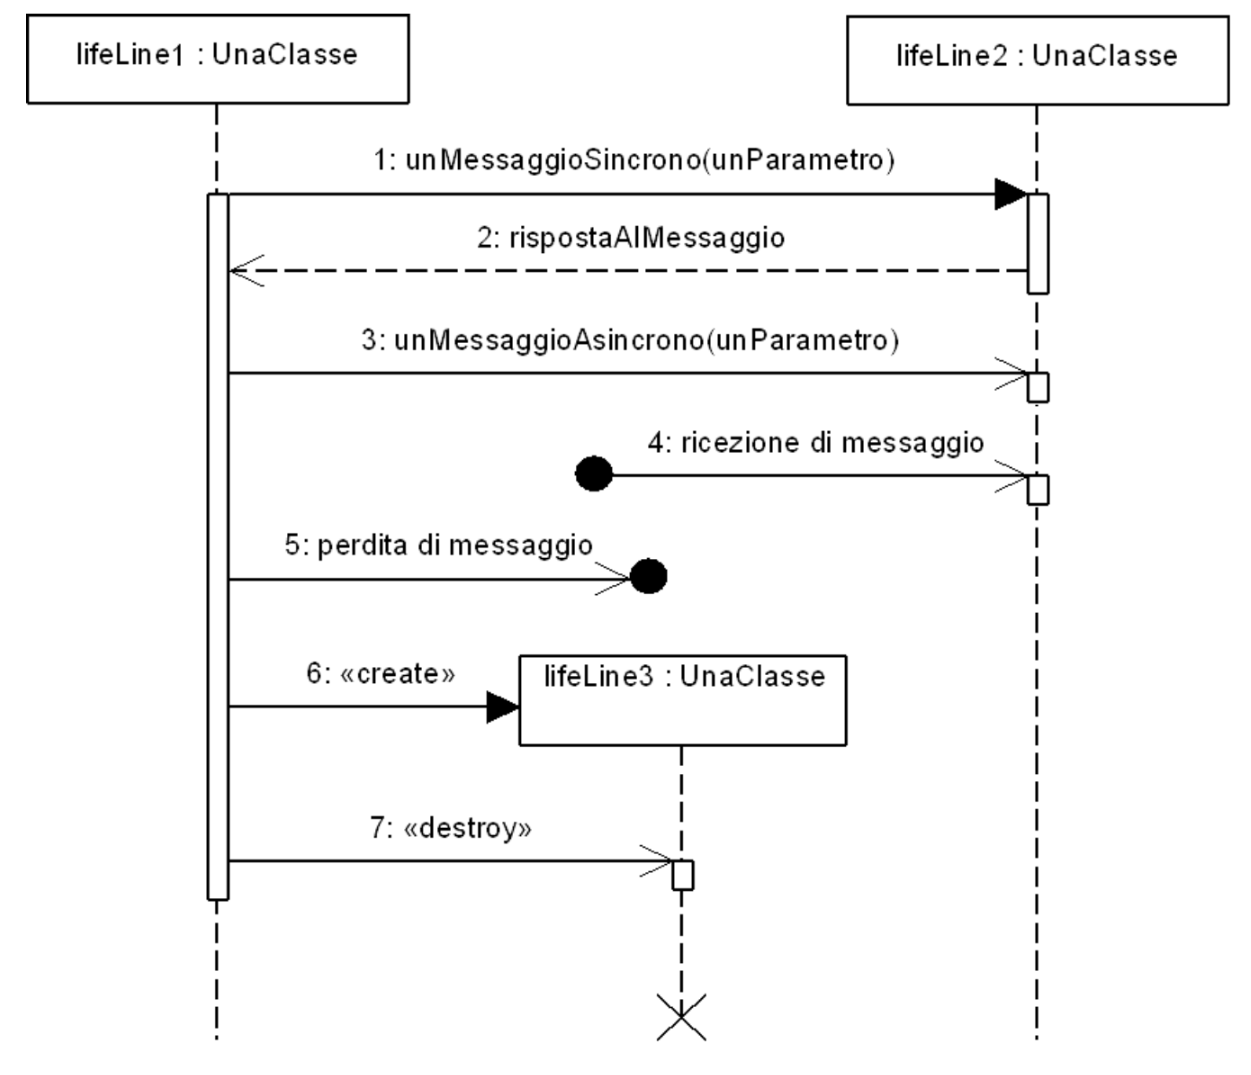
\includegraphics[scale=0.4]{../figures/lifeline_mess.png}
\end{center}

\subsubsection{Frammenti combinati}
I diagrammi di sequenza possono essere suddivisi in “aree” dette \textbf{frammenti combinati}.
Ogni frammento combinato ha un operatore, uno o più operandi e zero o più condizioni di guardia.

L'\textbf{operatore} determina come gli operandi vengono eseguiti: solitamente gli operatori ricalcano i costrutti dei linguaggi strutturati o altre caratteristiche dell'operazioni che vengono svolte (ad esempio esecuzione \textit{parallela}, \textit{atomica}, ecc...).

\newpage

La sintassi in UML sarà quindi la seguente:
\begin{center}
	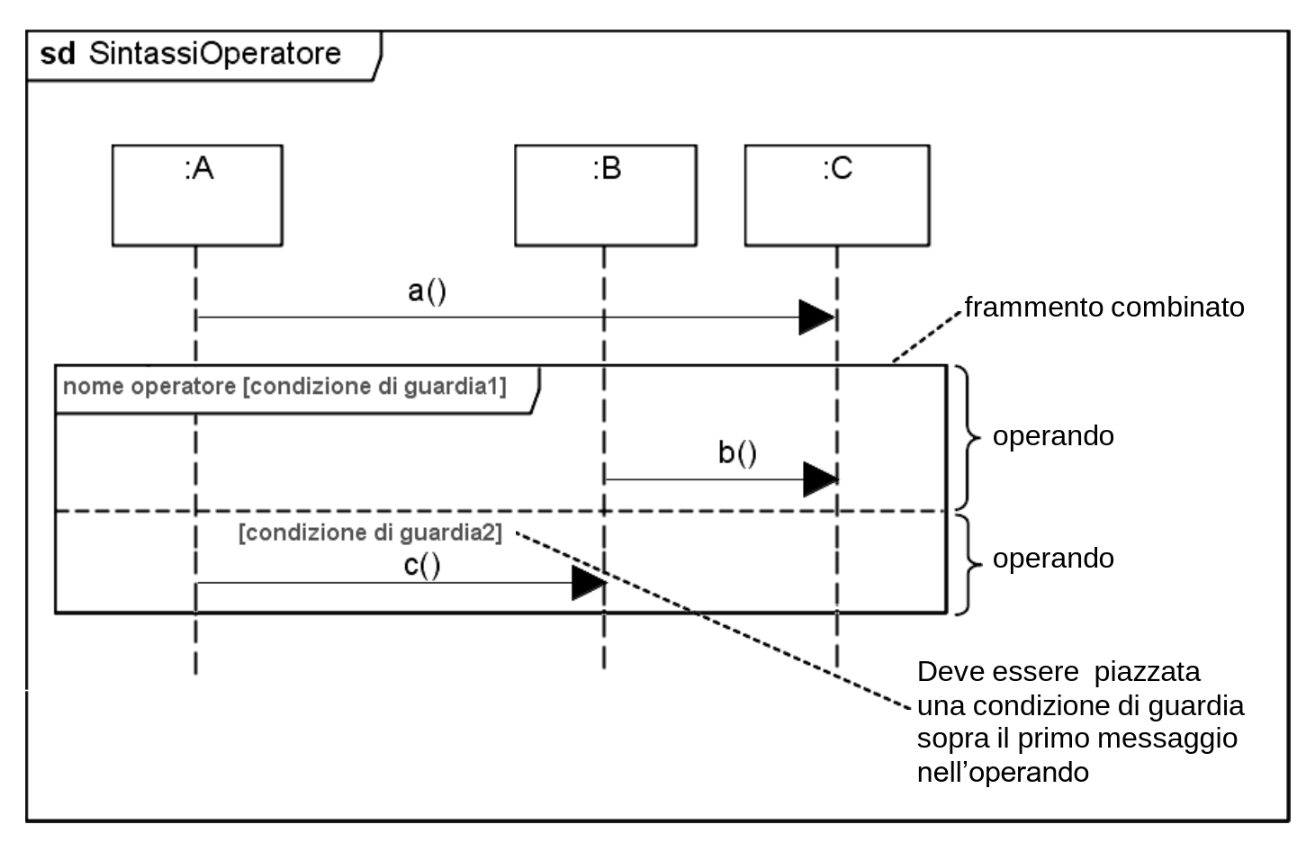
\includegraphics[scale=0.4]{../figures/frammenti_comb.png}
\end{center}

Vediamo una tabella che riassume gli operatori principali:
\begin{table}[H]
	\center \rowcolors{2}{white}{black!10}
	\begin{tabular} { c | c | p{9cm} }
		\bfseries Operatore & \bfseries Nome & \bfseries Significato \\
		\hline 
		\lstinline|opt| & opzione & Se la condizione è vera, viene eseguito un singolo operando \\ 
		\lstinline|alt| & alternative & L’operando la cui condizione è vera viene eseguito \\ 
		\lstinline|loop| & loop & Cicla max-min volte mentre la condizione è vera \\ 
		\lstinline|break| & break & Se la condizione di guardia è vera, l’operando è eseguito, ma non il resto dell’interazione \\ 
		\lstinline|ref| & riferimento & Il frammento combinato si riferisce ad un’altra interazione \\ 
		\lstinline|par| & parallelo & Tutti gli operandi vengono eseguiti in parallelo \\ 
		\lstinline|critical| & critico & L’operando viene eseguito atomicamente \\ 
		\lstinline|seq| & sequenza debole & Tutti gli operandi vengono eseguiti in parallelo con il vincolo che gli eventi che arrivano sulla stessa linea di vita da operandi differenti avvengano nella stessa sequenza degli operandi \\ 
		\lstinline|strict| & sequenza stretta & Gli operandi vengono eseguiti in stretta sequenza
	\end{tabular}
\end{table}

L'operatore \lstinline|loop| in particolare prevede più sintassi che rappresentano diversi tipi di iterazioni:
\begin{itemize}
	\item Loop for, che possono essere numerati;
	\item Loop while, che possono essere infiniti o fino a condizione non soddisfatta;
	\item Loop for-each, che possono essere ripetuti su collezioni o classi.
\end{itemize}

\subsubsection{Occorrenze di interazione}
Per evitare di ripetere più volte gli stessi frammenti di interazione, l'UML  mette a disposizione il riferimento ad interazione, detto \textbf{occorrenza di interazione} (che abbiamo visto come operatore \lstinline|ref|).

Questo può essere usato per riferirsi a frammenti di interazione in altri diagrammi di interazione.

\subsubsection{Parametri}
Le interazioni possono essere \textbf{parametrizzate}.
Questo permette di fornire valori diversi all'interazione ad ognuna delle sue occorrenze (meccanismo simile al passaggio di argomenti).

A scopo di esempio vediamo le interazioni parametrizzate \textit{TrovaStudente} e \textit{TrovaCorso} di un sistema di gestione univeristario:
\begin{center}
	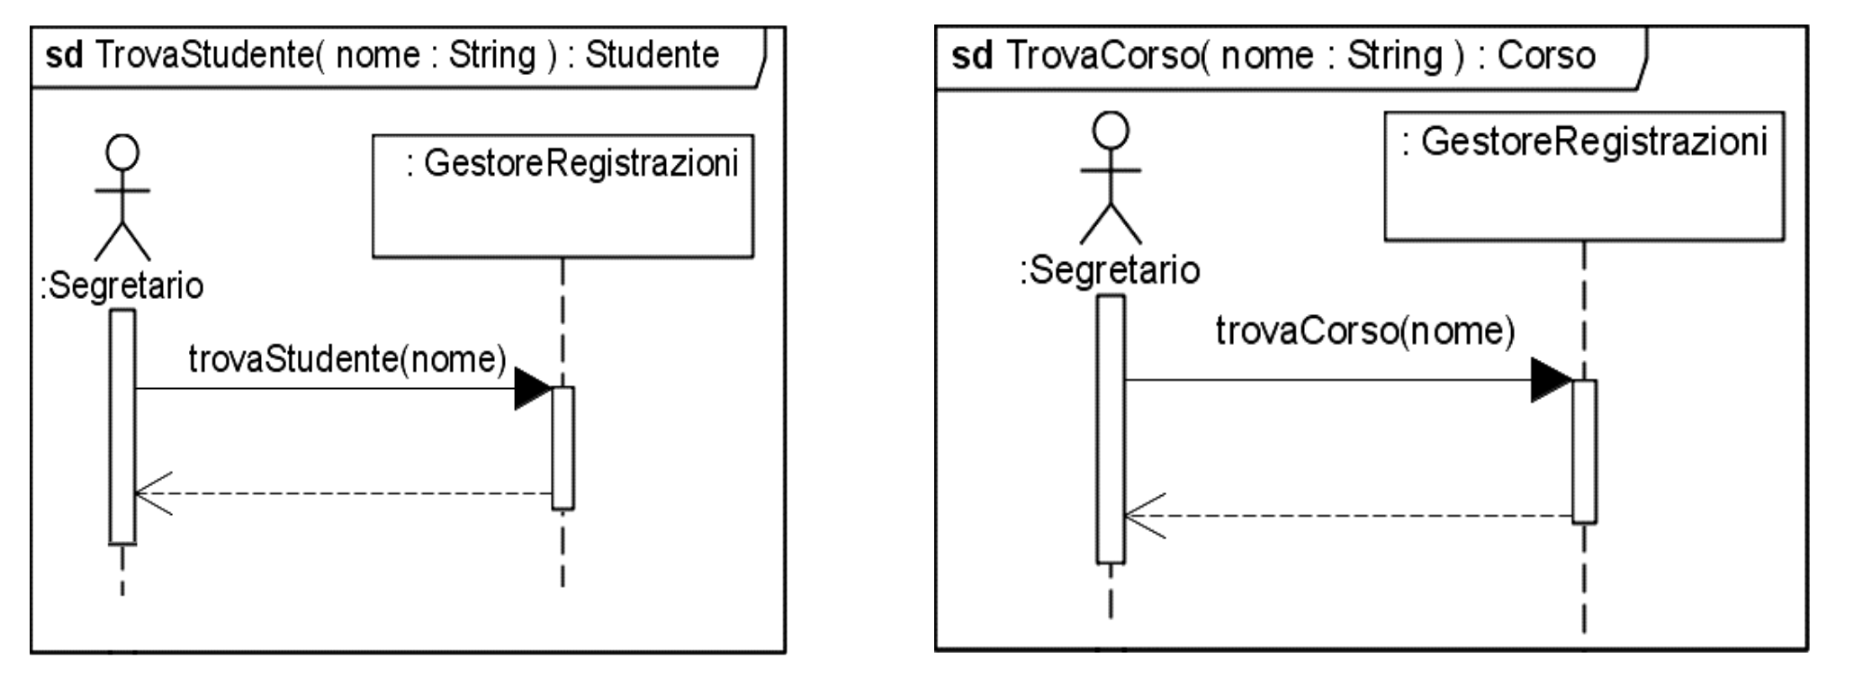
\includegraphics[scale=0.3]{../figures/frammenti_param.png}
\end{center}

\subsubsection{Gate}
I \textit{cancelli} (\textbf{gate}) rappresentano vie di accesso alle interazioni dall'esterno. Vengono quindi usati quando un’interazione è attivata da una linea di vita che non è parte dell’interazione stessa.

Vengono rappresentati graficamente come entrate ed uscite sulla finestra dell'interazione: questi punti connettono messaggi fuori dall'interazione a messaggi dentro l'interazione.

Sempre nel contesto dell'esempio sompra, vediamo come le interazioni viste possono essere realizzate anche coi gate:
\begin{center}
	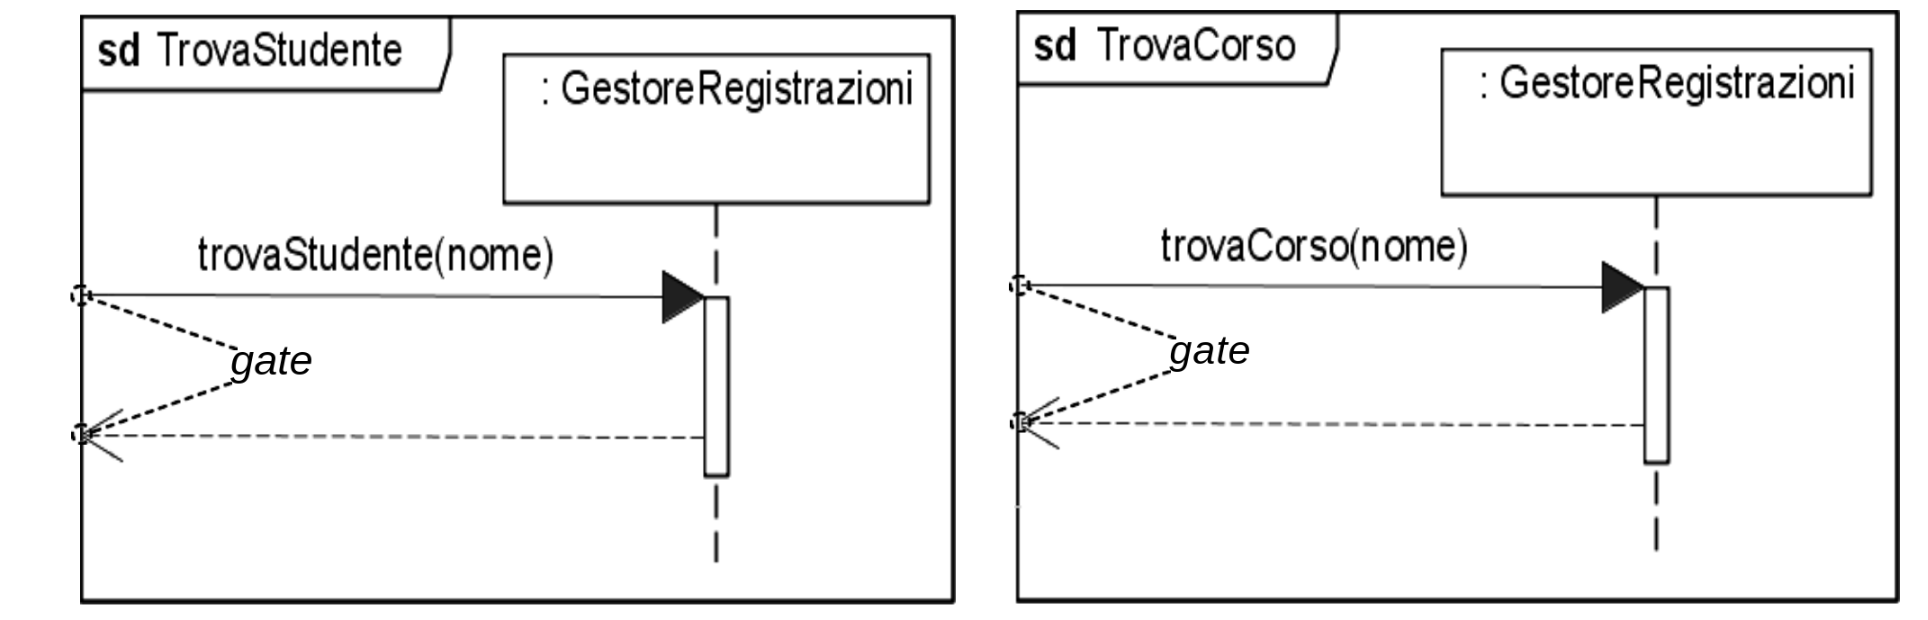
\includegraphics[scale=0.3]{../figures/frammenti_gate.png}
\end{center}

Il meccanismo dei gate potrebbe sembrare simile a quello dei parametri. In sostanza si può dire che:
\begin{itemize}
	\item I parametri rappresentano bene informazioni note all'interno dell'interazione;
	\item I gate rappresentano invece informazioni che provengono dall'esterno dell'interazione.
\end{itemize}

\subsection{Workflow progetto}
L'obiettivo del workflow \textbf{progetto} è approfondire la fase di \textit{design} del sistema: qui si devono definire completamente tutte le funzionalità implementate per soddisfare i requisiti dell'utente.

Abbiamo studiando nel workflow \textit{requisiti} come estrapolare i requisiti dal sistema dal dominio di sua applicazione; nel workflow \textit{analisi} abbiamo esplorato il dominio del problema in modo da modellare strutture di classe e interazioni; adesso vogliamo tradurre questi modelli in soluzioni tecniche vere e proprie.

Abbiamo che questo workflow è tipico della fase di \textit{elaborazione} e \textit{costruzione} del software vero e proprio.

\subsubsection{Classi di progetto}
Di base, per ogni \textit{classe di analisi} ci sono una o più \textbf{classi di progetto}, e opportunamente delle \textit{interfacce}:
\begin{center}
	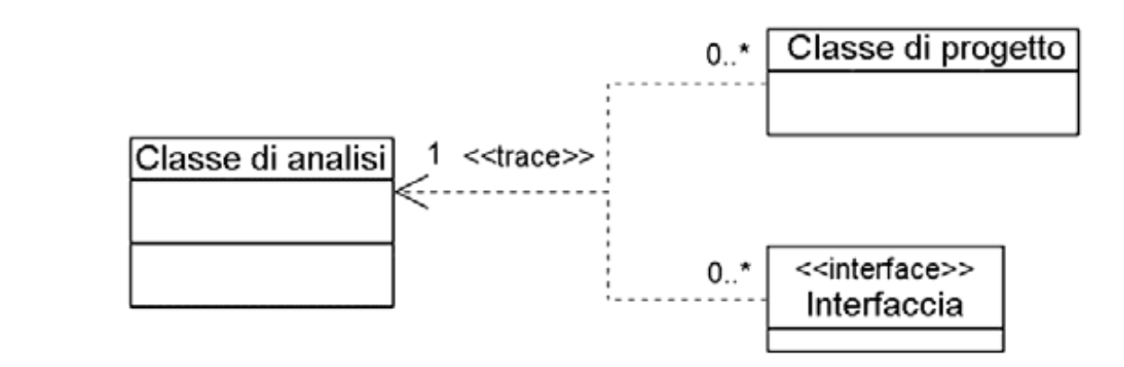
\includegraphics[scale=0.4]{../figures/classi_analisi_progetto.png}
\end{center}

Queste non hanno più il solo scopo di modellare il dominio di problema, ma anche di essere realizzabili da programmatori veri e propri. 

Abbiamo quindi che sono influenzate da:
\begin{itemize}
	\item Il \textbf{dominio di problema}: come abbiamo visto raffinando le classi di analisi attraverso dettagli implementativi;
	\item Il \textbf{dominio della soluzione}: composto dall'insieme di \textit{librerie}, \textit{database}, \textit{interfacce} e altre tecnologie che verranno adottate per l'implementazione vera e propria.
\end{itemize}

Campi e metodi delle classi di progetto devono essere completamente definiti (e implementabili). Per i campi, si può iniziare a specificare i tipi di variabile (se applicabile), per i metodi tipi di argomenti e ritorno.
Opportunamente, è meglio dividere classi in più sottoclassi che \textit{"ingigantire"} una classe fino a renderla inutilizzabile.

Una classe di progetto è ben definita quando risulta:
\begin{itemize}
	\item \textbf{Completa} e \textbf{sufficiente}: le operazioni pubbliche della classe definiscono un \textit{contratto} ben chiaro e definito con i clienti della stessa.
		Una classe è completa quando offre ai suoi clienti tutto quello che i clienti si aspettano, senza operazioni in più (che non rientrano nel dominio di competenza della classe) e senza operazioni in meno (cosa che non onererebbe il contratto);
	\item \textbf{Primitiva}: le classi non dovrebbero implementare lo stesso comportamento più volte: dovrebbero fornire servizi singoli e atomici;
	\item \textbf{Alta coesione}: le classi dovrebbero modellare un singolo concetto astratto e contenere campi e metodi direttamente riconducibili a quel concetto astratto;
	\item \textbf{Basso accoppiamento}: le classi dovrebbero essere associate in interazioni con le sole classi con cui dividono \textit{responsabilità}. Di base, non conviene usare metodi di altre classi solo perché il codice verrebbe altrimenti ripetuto: meglio non sacrificare la solidità strutturale per scrivere meno righe.
\end{itemize}

\subsubsection{Ereditarietà}
In analisi, si usa la relazione di erediterietà se si vuole modellizzare una relazione "is a" chiara e definita.
In fase di progetto, l'ereditarietà scoperta in fase di analisi può essere usata per rafforzare la struttura delle classi e risparmiare codice per funzioni a queste comuni.

\subsubsection{Classi annidate}
Le classi annidate sono specifiche ad alcuni linguaggi come il Java. Solitamente sono sconsiliate in quanto non ci permettono di distinguere facilmente chi sta dando problemi fra la classe madre e la classe annidata. 

\subsubsection{Relazioni fra classi di progetto}
Veniamo al problema di rendere le \textbf{relazioni} fra classi (cioè le \textit{associazioni}) in un'implementazione in fase di progetto.

Partiamo dall'idea che nei linguaggi di progammazione che consideriamo (OOP standard, come Java o C++), non c'é nessun modo di rendere relazioni bidirezionali, o relazioni molti a molti.

Dobbiamo quindi seguire delle procedure per trasformare le associazioni di questo tipo in associazioni implementabili nel nostro dominio di soluzione.

Queste procedure possono essere:
\begin{itemize}
	\item Trasformare associazioni in relazioni di \textbf{aggregazione} o \textbf{composizione} dove appropriato:

		\begin{itemize}
			\item La relazione di \textbf{aggregazione} è una relazione lieve fra oggetti, che lega una parte ad un'intero dove l'intero è composto da molte parti.
Le parti dell'intero sono in qualche modo autosufficienti, ed esistono a priori di questo.

Un esempio di aggregazione è la relazione fra un computer e le sue parti:
\begin{center}
	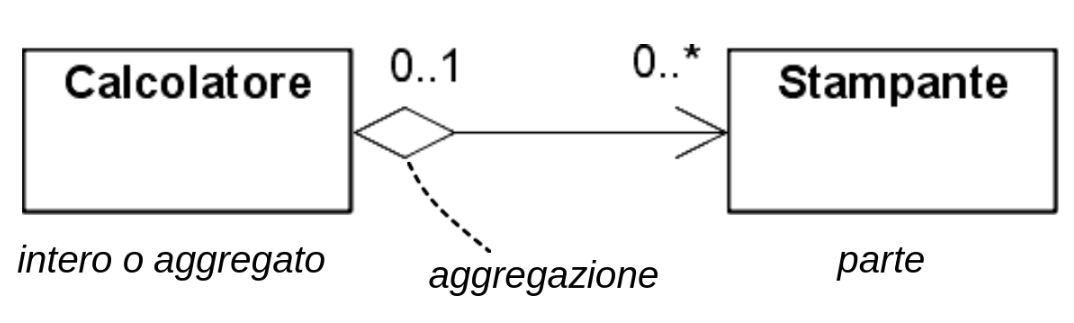
\includegraphics[scale=0.3]{../figures/aggregazione.png}
\end{center}

			\item La relazione di \textbf{composizione} è di contro una relazione molto forte, dove la parte esiste in funzione dell'intero. Ad esempio, in questo caso se muore la parte muore anche l'intero.

	Un esempio di composizione è la relazione fra la parte del computer e i suoi componenti:
\begin{center}
	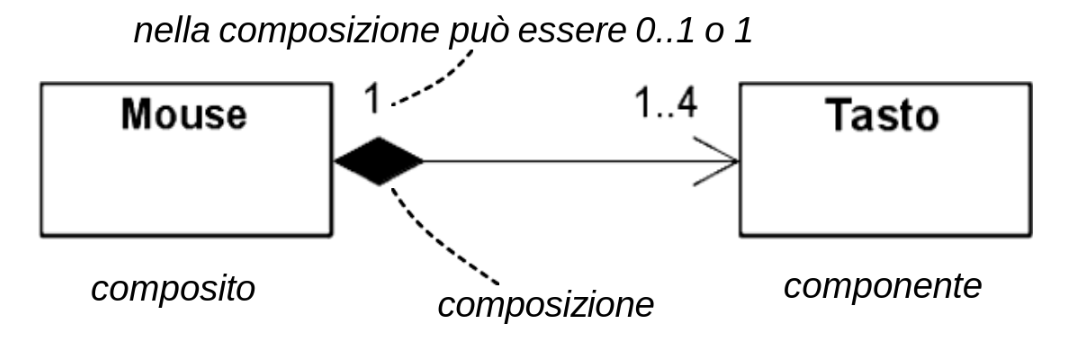
\includegraphics[scale=0.3]{../figures/composizione.png}
\end{center}
		\end{itemize}

		Chiaramente, bisogna distinguere prima chi nella relazione è la parte e chi l'intero, e poi risolvere problemi come capire le molteplicità (lato intero, da 0 a 1 si può comporre, oltre bisogna aggregare).

	\item Implementare associazioni uno-a-uno: questo si può fare sia per composizione che per aggregazione.
		Ad esempio:
\begin{center}
	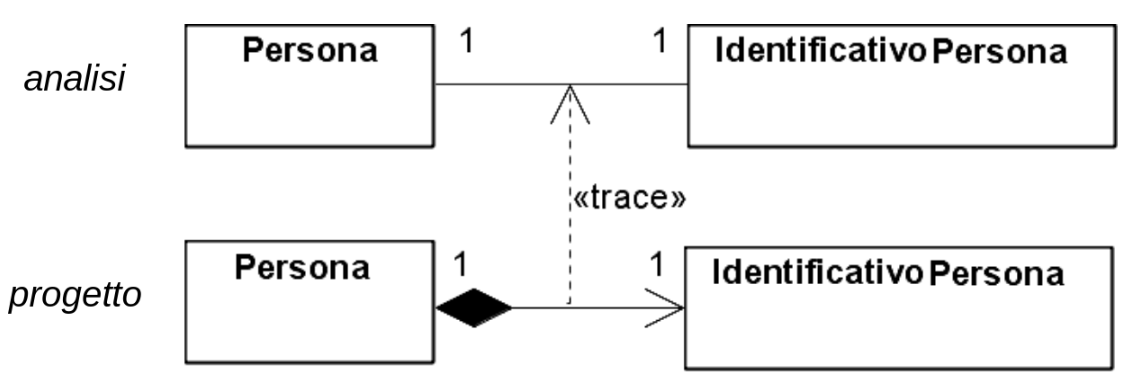
\includegraphics[scale=0.3]{../figures/uno-uno.png}
\end{center}

	\item Implementare associazioni molti-a-uno: questo si fa solitamente per aggregazione, prendendo le \textit{molte} parti come aggregate all'\textit{uno}.
		Ad esempio:
\begin{center}
	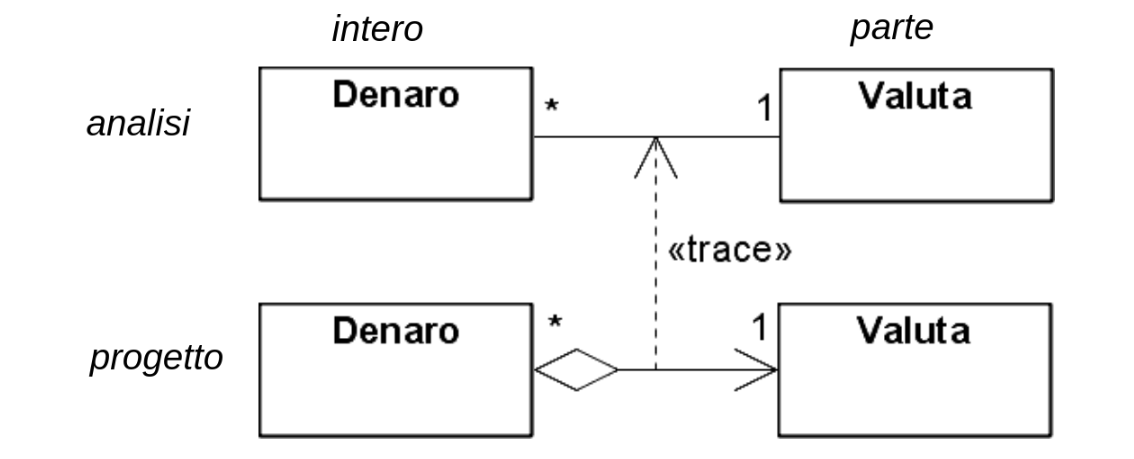
\includegraphics[scale=0.3]{../figures/molti-uno.png}
\end{center}

	\item Implementare associazioni uno-a-molti: qui bisogna usare una classe \textit{collezione} esplicita, come ad esempio un vettore.
		
		Vediamo infatti il confronto fra la relazione molte a molti in fase di analisi alla sua implementazione in fase di progetto:
\begin{center}
	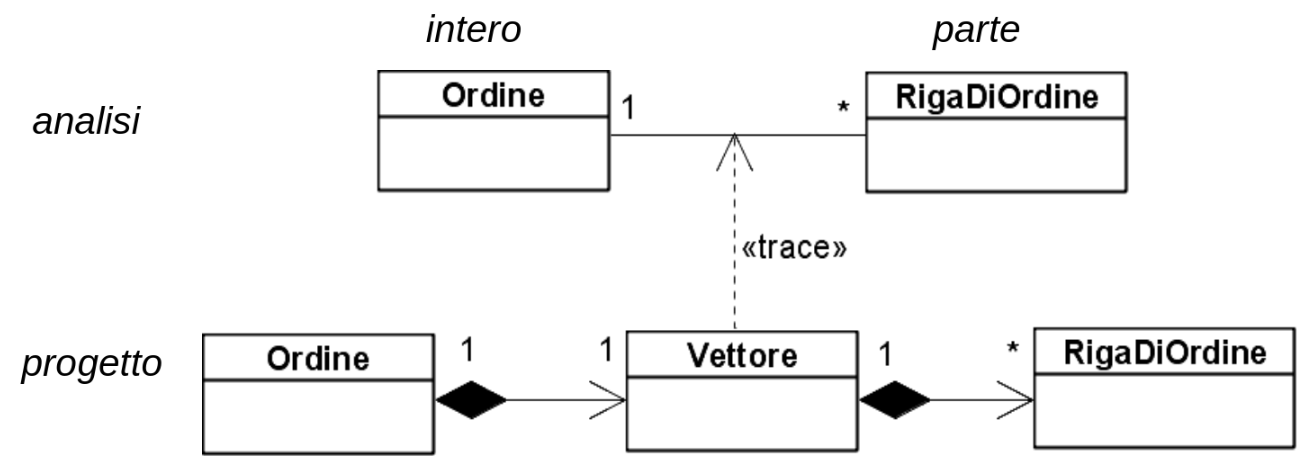
\includegraphics[scale=0.3]{../figures/uno-molti.png}
\end{center}


	\item Implementare associazioni molti-a-molti;
	\item Implementare associazioni bidirezionali;
	\item Implementare classi di associazioni.
\end{itemize}

\subsection{Realizzazione casi d'uso di progetto}
Come per le classi di analisi, anche i casi d'uso vanno rielaborati in \textbf{casi d'uso di progetto}:
\begin{center}
	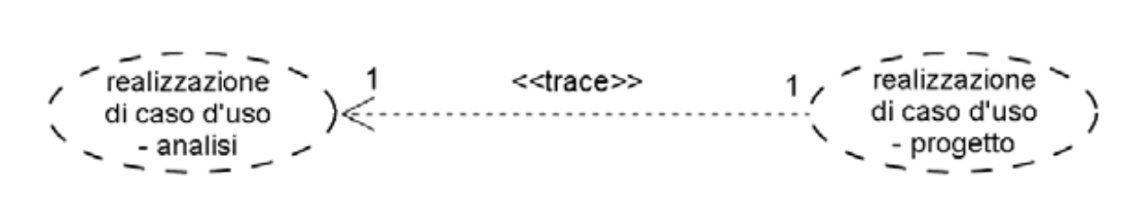
\includegraphics[scale=0.4]{../figures/casi_uso_analisi_progetto.png}
\end{center}
Rispetto all'attività corrisondente in fase di analisi, abbiamo in fase di progetto alcune differenze:
\begin{itemize}
	\item La realizzazione dei casi d'uso coinvolge l'uso di di classi progetto, interfacce e componenti piuttosto che classi d'analisi;
	\item Il processo di creazione di realizzazione di casi d'uso di progetto scoprirà nuovi requisiti non funzionali e classi di progetto (atti ad interagire con il dominio della soluzione);
	\item Le realizzazioni dei casi d'uso aiutano a trovare i \textbf{meccanismi centrali}, cioè modi standard di risolvere un particolare problema di progetto che sono applicati consistemente nello sviluppo del sistema. 
\end{itemize}

Una realizzazione di un caso d’uso nel progetto consiste in \textbf{diagrammi di interazione} e \textbf{diagrammi delle classi}.

\subsection{Workflow implementazione}
Veniamo quindi all'implementazione effettiva del sistema progettato in fase di progetto. Chiave di questo workflow è la scrittura di \textbf{codice}, \textbf{testing} estensivo di ogni singola funzionalità che si vuole produrre, e \textbf{dislocazione} su un'architettura reale del sistema sviluppato.

\newpage

Vediamo un diagramma che spiega come vogliamo associare al modello realizzato in fase di progetto un \textit{implementaione} vera e propria:
\begin{center}
	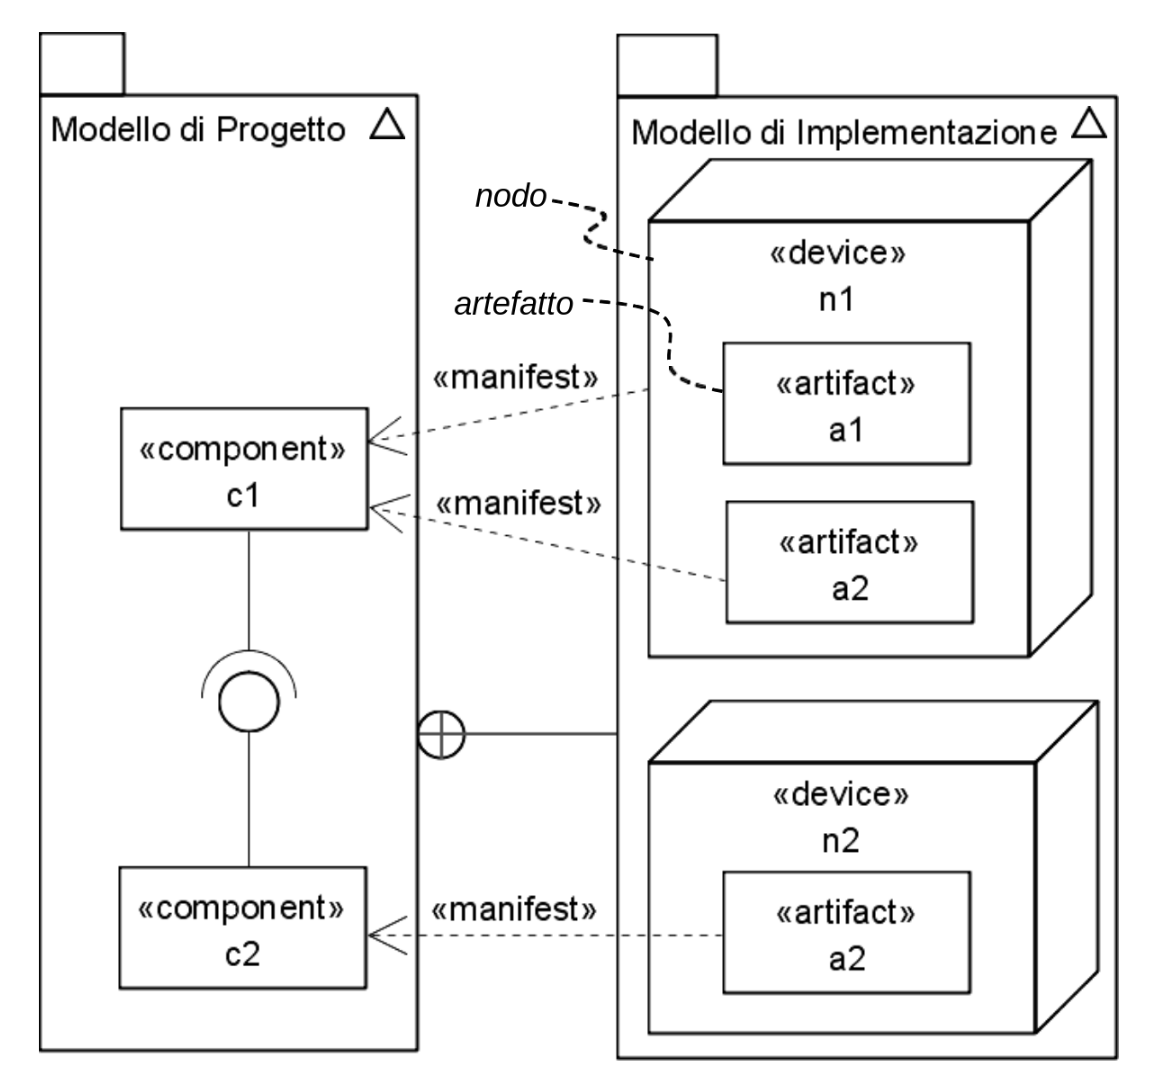
\includegraphics[scale=0.4]{../figures/implementazione.png}
\end{center}
Nell'esempio, la relazione \lstinline|<<manifest>>| significa che i componenti d'implementazione, appunto, \textit{implementano} i relativi componenti della fase di progetto.

Solitamente nella fase di implementazione questa fase non è più necessario modellare ulteriori componenti.
Eccezioni potrebbero essere le situazioni:
\begin{itemize}
	\item Si vuole generare il codice direttamente dal modello;
	\item Se si sta organizzando uno sviluppo basato sui componenti (\textit{Component Based Development}): in questo caso scegliere come disporre i componenti diventa un problema strategico.
\end{itemize}

Gli artefatti che vogliamo generare sono:
\begin{itemize}
	\item \textbf{Diagrammi di componenti} che mostrano come gli artefatti rendono manifesti i componenti implementati;
	\item \textbf{Diagrammi di dislocazione} che rappresentano come gli artefatti vengono fisicamente dislocati su architetture reali per implementare il servizio richiesto. 
\end{itemize}

\subsection{Diagrammi di dislocazione}
I diagrammi di dislocazione rappresentano come gli artefatti prodotto vengono, appunto, \textit{dislocati} su istanze di nodi (macchine, ecc...).
Questo processo è estremamente importante ad esempio nello sviluppo di architetture distribuite.

Esistono 2 tipi di diagrammi di dislocazione:
\begin{itemize}
	\item \textbf{Descrittivi}: contiene nodi ed artefatti, e le relazioni che vi avvengono. Un nodo è una macchina, mentre un'artefatto è software in esecuzione su tale macchina; 
	\item \textbf{D'istanza}: contengono istanze di nodi, di artefatti, e di relazioni. Qui le istanze di nodi sono macchine specifiche, le istanze di artefatti sono processi specifici, e così via. 

		Comunque, è possibile usare nodi e artefatti anonimi quando il loro comportamento è noto a prescindere dalla specificità. 
\end{itemize}

Vediamo quindi l'esempio di un diagramma di dislocazione, \textit{d'istanza}, relativo ad un'applicazione distribuita:
\begin{center}
	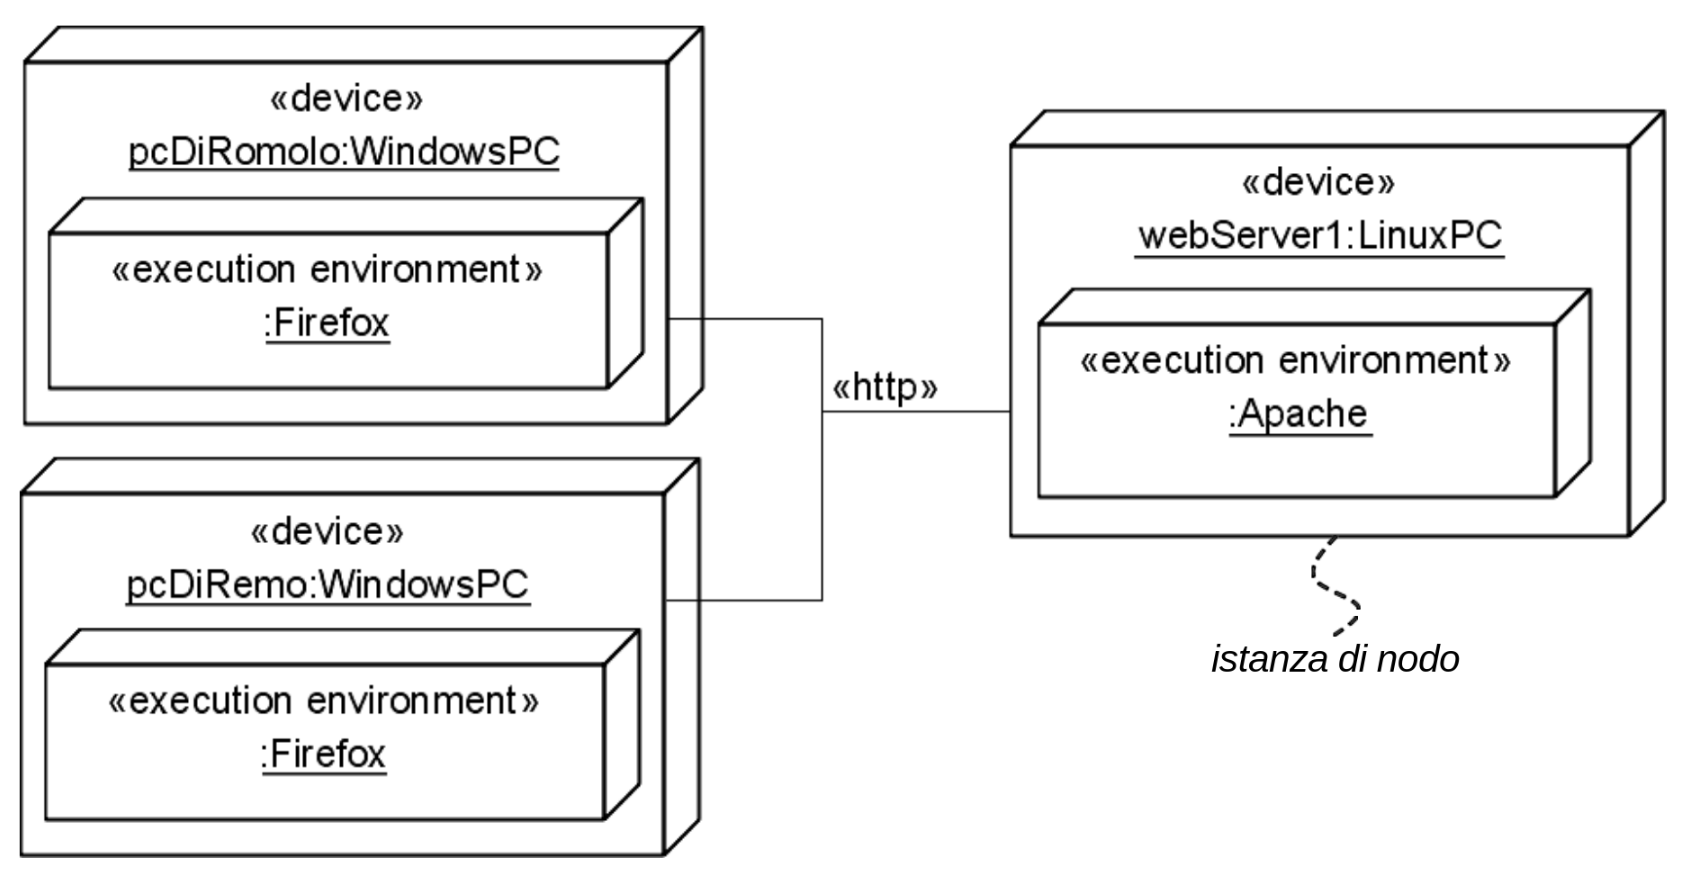
\includegraphics[scale=0.3]{../figures/dislocazione.png}
\end{center}

\subsubsection{Nodi}
In dettaglio, i \textbf{nodi} rappresentano risorse computazionali che possono essere usate per realizzare il servizio. Ne distinguiamo 2 tipi:
\begin{itemize}
	\item \lstinline|<<device>>|: nodi che rappresentano dispositivi fisici;
	\item \lstinline|<<execution environment>>|: nodi che rappresentano ambienti di esecuzione per software.
\end{itemize}

Le \textbf{associazioni} fra nodi e artefatti sono a questo punto canali di comunicazione dove informazioni possono essere scambiate.

\subsubsection{Artefatti}
Gli artefatti rappresentano lato software tutto ciò che viene effettivamente implementato, fra cui:

\begin{itemize}
	\item File sorgenti;
	\item File eseguibili;
	\item Script;
	\item Tabelle di basi di dati;
	\item Documenti;
	\item Risultati del processo di sviluppo.
\end{itemize}

\subsection{Workflow test}
Veniamo quindi a discutere l'attività di \textbf{testing} che è opportuno applicare durante e dopo lo sviluppo.

Sappiamo che è impensabile sviluppare software privo di errori.
Per questo dobbiamo:
\begin{itemize}
	\item Testare il software spesso;
	\item Scrivere software che sia facile da testare.
\end{itemize}

\subsubsection{Operazioni di test}
La fase di testing si effettua vari livelli e consiste in operazioni distinte:
\begin{itemize}
	\item Test di \textbf{unità};
	\item Test di \textbf{modulo};
	\item Test di \textbf{sottosistema};
	\item Test di \textbf{sistema} o \textbf{integrazione};
	\item Test \textbf{alfa}: prima fase dove si fornisce il sistema al cliente;
	\item Test \textbf{beta}: seconda fase, in cui si fornisce il sistema a più utenti;
	\item Test \textbf{benchmark}: il sistema viene testato in maniera standardizzata per valutarne le prestazioni;
	\item Test di \textbf{stress}: il sistema viene messo al prova in termini di resilienza, sicurezza, ecc... sopponendolo ad attachi o comunque stress.
\end{itemize}

\subsubsection{Testing e debugging}
Testing e debugging sono processi diversi fra di loro ma legati:
\begin{itemize}
	\item Il \textbf{testing} serve a valutare la presenza di un errore;
	\item Il \textbf{debugging} è l'atto di risolvere tale errore.
\end{itemize}

I test di \textbf{regressione} sono utili dopo il debugging, per confermare che l'attività di debugging non abbia prodotto ulteriori errori.

\subsubsection{Distribuzione di errori}
Gli errori, come abbiamo detto, si verificano a prescindere dalle nostre migliori intenzioni.
Possiamo adottare alcune euristiche per capire come sono distribiti:
\begin{itemize}
	\item Gli errori tendono a concentrarsi in moduli \textbf{specifici}, solitamente i \textit{più complessi};
	\item Un modulo che contiene un errore probabilmente ne conterrà altri;
	\item Moduli strettamente accoppiati condivideranno più errori;
	\item Moduli che vengono rielaborati spesso (\textit{refactoring} o \textit{manutenzione}) sono più facilmente soggetti ad errori, sopratutto man di mano che il processo di refactoring si prolunga nel tempo.
\end{itemize}

\end{document}
